\section*{Diagramas de Penrose}
\underline{Métrica de Minkowski} \text{(adimensional, esféricas, d$\theta$ =0):}
\begin{align*}
    &\text{Cuadrimomento de la luz: }\underline{k}=A\, e_0+\sqrt{A^2-\frac{B^2}{r^2}}\,e_1+\frac{B}{r^2}\,e_3\\
    &\frac{dt}{d\lambda}=A\; \; \; \; \frac{dr}{d\lambda}=\sqrt{A^2-\frac{B^2}{r^2}}\; \; \; \; \frac{d\phi}{d\lambda}=\frac{B}{r^2}\; \Rightarrow\; \text{Geodésica: }t-t_0=\pm\sqrt{r^2-\frac{B^2}{A^2}}\\
    &\text{Aunque al graficar las geodésicas obtengamos curvas, debemos recordar que es un}\\
    &\text{efecto causado por la elección de las coordenadas, pues la luz se mueve en línea}\\
    &\text{recta en el espacio-tiempo de Minkowski.}\\
    &\dashv \text{ Métrica en las coordenadas del Diagrama de Penrose: }\\
    &ds^2=\frac{-dT^2+dX^2}{[1-(T+X)^2]\,[1-(T-X)^2]}\;\; \; \left|
    \begin{array}{ll}
         &\hspace{-12pt}    u=T+X\\
         &\hspace{-12pt}    v=T-X
    \end{array}
    \right.
    \;\;  \left|
    \begin{array}{ll}
         &\hspace{-12pt}    u=\tanh q\\
         &\hspace{-12pt}    v=\tanh p
    \end{array}
    \right.
    \; \left|
    \begin{array}{ll}
         &\hspace{-12pt}    p=t-r\\
         &\hspace{-12pt}    q=t+r
    \end{array}
    \right.\\
    &\text{Restringido a: }X\geq0\; \; \; -1<T+X<1 \; \; \;-1<T-X<1
\end{align*}
\vspace{-5pt}
\begin{minipage}{0.35\textwidth}
    $\bullet \; \text{Diagrama de Penrose para el espacio-tiempo de Minkowski}$
    
    \centering
    \scalebox{0.7}{
    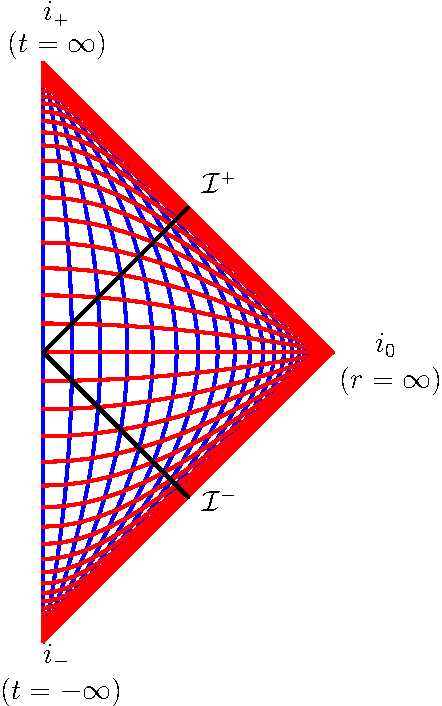
\includegraphics[height=200pt]{sections/F2_penrose_diag.pdf}
    }
\end{minipage}
\underline{Métrica de Kruskal} \text{(esféricas, d$\Omega$ =0):}
\begin{align*}
        &\dashv \text{ Métrica en las coordenadas del Diagrama de Penrose: }\\
    &ds^2=\frac{1}{r}e^{-r}(1+q^2)(1+p^2)[-d\mathcal{T}^2+d\mathcal{R}^2]\; \; \left|
    \begin{array}{ll}
         &\hspace{-12pt}    \mathcal{T}\!=\!u+\!v\\
         &\hspace{-12pt}    \mathcal{R}\!=\!u\!-\!v
    \end{array}
    \right.
    \hspace{-2pt}
  \left|
    \begin{array}{ll}
         &\hspace{-12pt}    u\!=\!\arctan q\\
         &\hspace{-12pt}    v\!=\!\arctan p
    \end{array}
    \right.
    \hspace{-2pt}
    \left|
    \begin{array}{ll}
         &\hspace{-12pt}    p\!=\!T\!-\!X\\
         &\hspace{-12pt}    q\!=\!T\!+\!X
    \end{array}
    \right.
\end{align*}
\begin{minipage}{0.3\textwidth}
    $\bullet \; \text{Diagrama de Penrose para el espacio-tiempo de Kruskal}$
        
    \centering
    \scalebox{0.75}{
    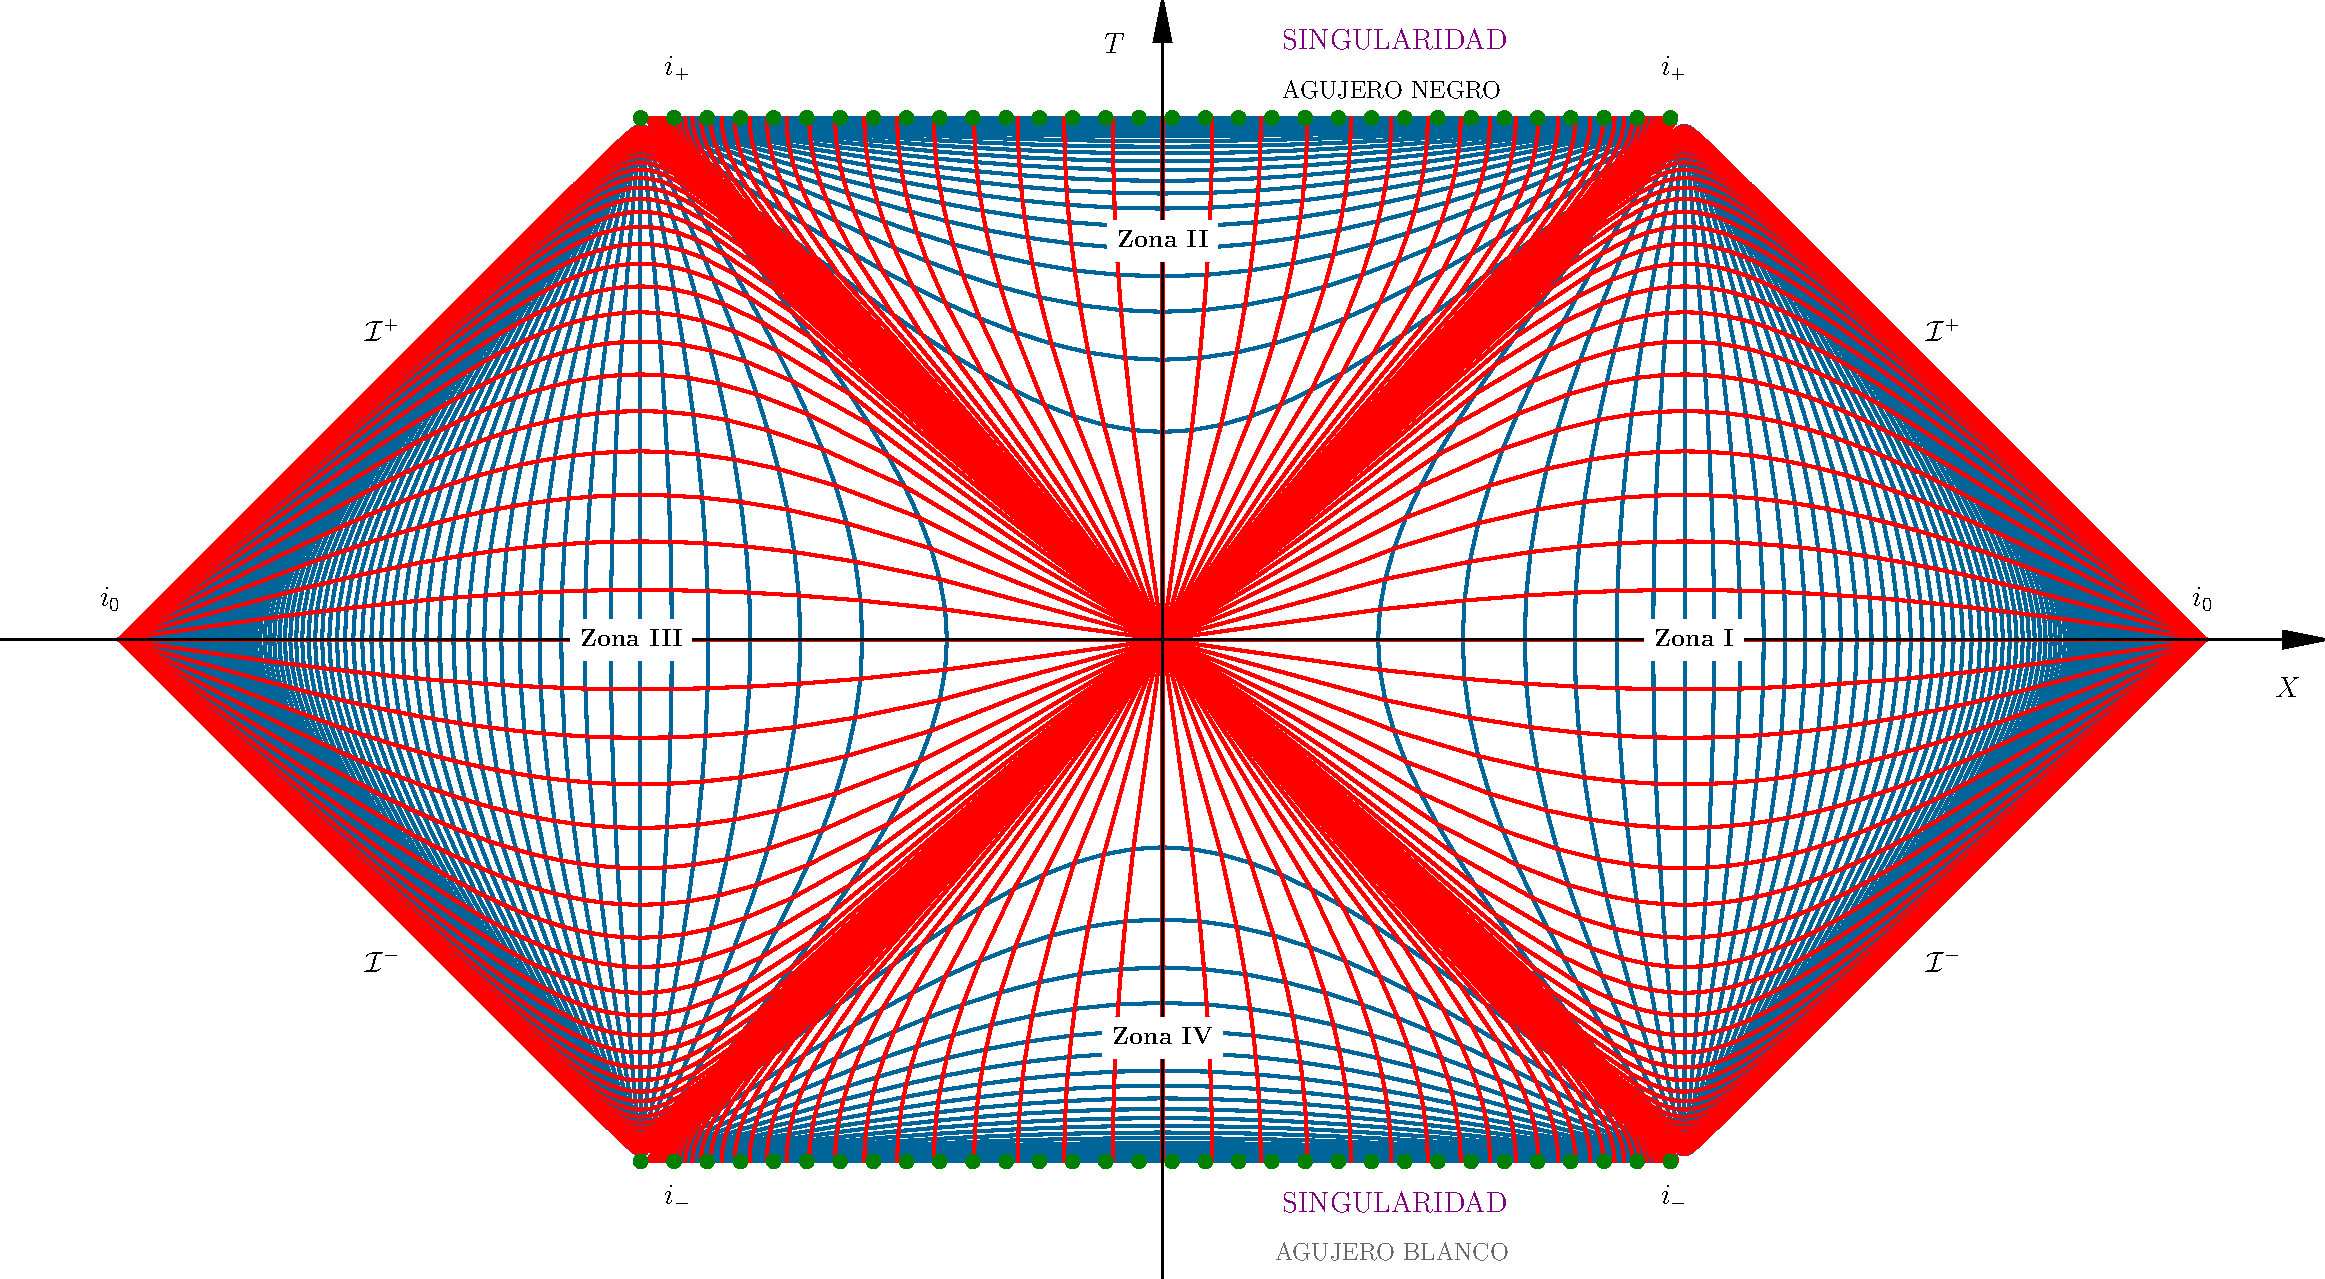
\includegraphics[height=200pt]{sections/F3_penrose_diag_schwar.pdf}
    }
\end{minipage}
\\
